\section{STEADY-STATE THERMAL ANALYSIS}
\normalsize{Steady-state thermal analysis is the main type of analysis that was carried out to analyse the different components of the \acrshort{ECRH} \acrshort{TZM}-reflector tile assembly. Different scenarios and loadcases were designed to give insight on the thermal behavior and performances of the tile, that being, the impact of the design changes of the \acrshort{TZM}-reflector tile, the influences of different \acrshort{ECRH} beam configurations or the influences of the film coefficient in the cooling pipe.}
\subsection{Calculation of the surface integrales}
\normalsize{To compare between the old and new tile design but also validate the finite element model, calculating the surface integral can be of use. This idea behind this is to check for energy conservation after integration the heat flux of the \acrshort{ECRH} beam on the tile surface. Analytical calculations are a good approach to estimate the overall heat flow through the \acrshort{TZM} tile. After the calculation of the surface integrales ($\it{see}$ \ref{MODELLING OF THE ECRH BEAM}), it is possible to numerically estimate an integral and predictict the heat flux through the old and the new design.}
\\
\break
\normalsize{\indent The surface onto which the heat disribution is integrated is a rough approximation of the surface of the \acrshort{TZM} tile (the projected area of the tile was simplified to a rectangle of size $95mm \times 95mm$). The function is then integrated using a Wolfram Mathematica\textsuperscript{\textregistered} script. To evaluate the validity of the analytical calculation, a finite element model including only the old and the new \acrshort{TZM} tile was developed to calculate the surface integral but using the finite element method. The idea is to compare both methods to estimate the heat flow. }
\\
\begin{figure}[h!]
    \label{fig_5_1} 
    \centering
    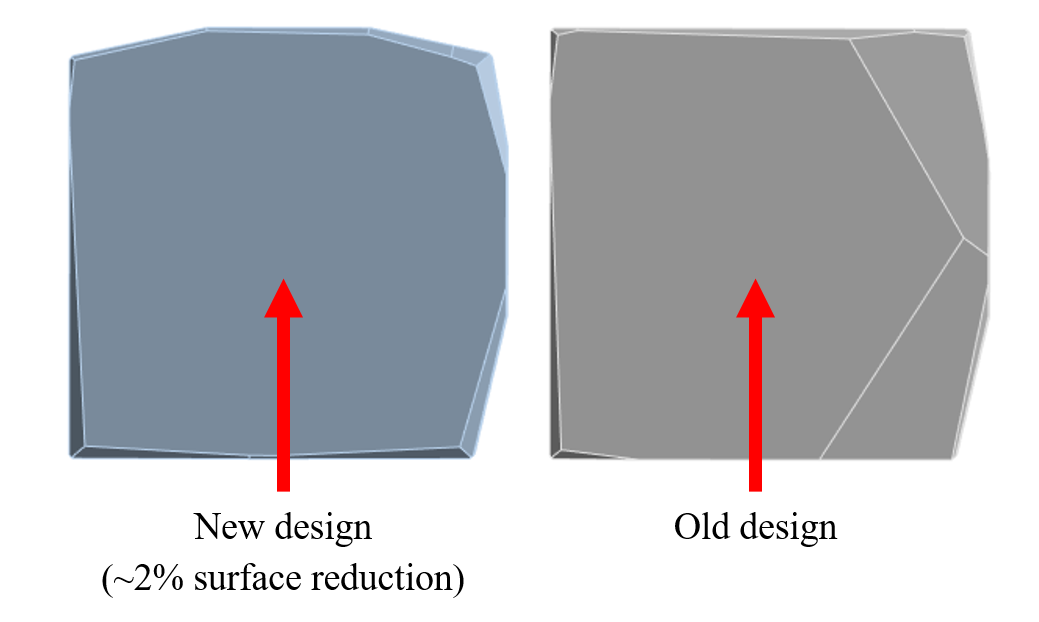
\includegraphics[width=.7\textwidth]{figures/standalonetilemodel.png}
    \caption{\it 3D model of the TZM tiles for integral calculation}
\end{figure}
\\
\break
\normalsize{\indent }
\subsection{Comparison between old and new TZM tile design}
\subsection{Film coefficient influence on thermal behavior}
\subsection{Loadcase influence on thermal behavior}